\documentclass[10pt,a4paper]{article}
\usepackage[utf8]{inputenc}
\usepackage{amsmath}
\usepackage{amsfonts}
\usepackage{amssymb}
\usepackage{listings}
\usepackage{graphicx}
\lstset{showstringspaces=false}
\begin{document}
\title{Intelligent Systems Assignment 1}
\author{Wessel Becker (1982362) \& Sander ten Hoor (2318555)}
\maketitle
\section{MatLab code}
\subsection{Changes to tsp.m}
The decrease T by 0.1\% was removed to make T a constant value.

\lstinputlisting[language=Matlab, firstline=27, lastline=29]{./Salesman/tsp.m}
\subsection{plotmean.m}
\lstinputlisting[language=Matlab]{./Salesman/plotmean.m}

\section{Plots}
To show the impact of the temperature, several values for the temperature have been used to run the tsp function. The tsp function returns the generated distance values. The last fifty of these values are used to plot the mean against the used temperature.

These plots show the value of the temperature on the x-axis against the mean normalised path distance on the y-axis. The standard deviation is displayed around the data points.

\makebox[\textwidth]{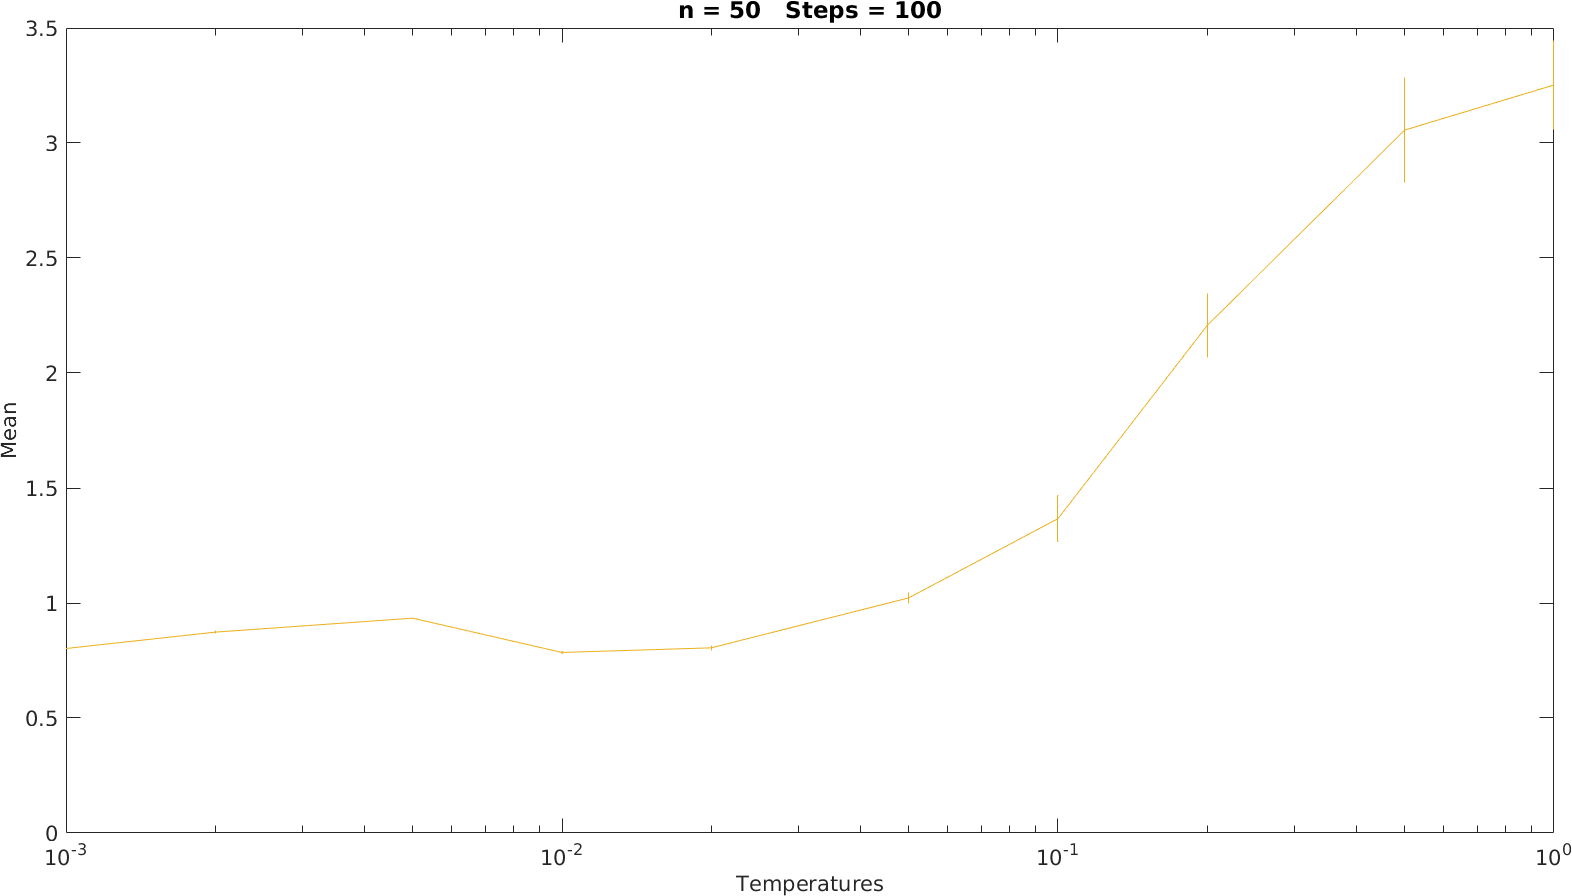
\includegraphics[width=\textwidth]{./Salesman/n50s100}} \\

\makebox[\textwidth]{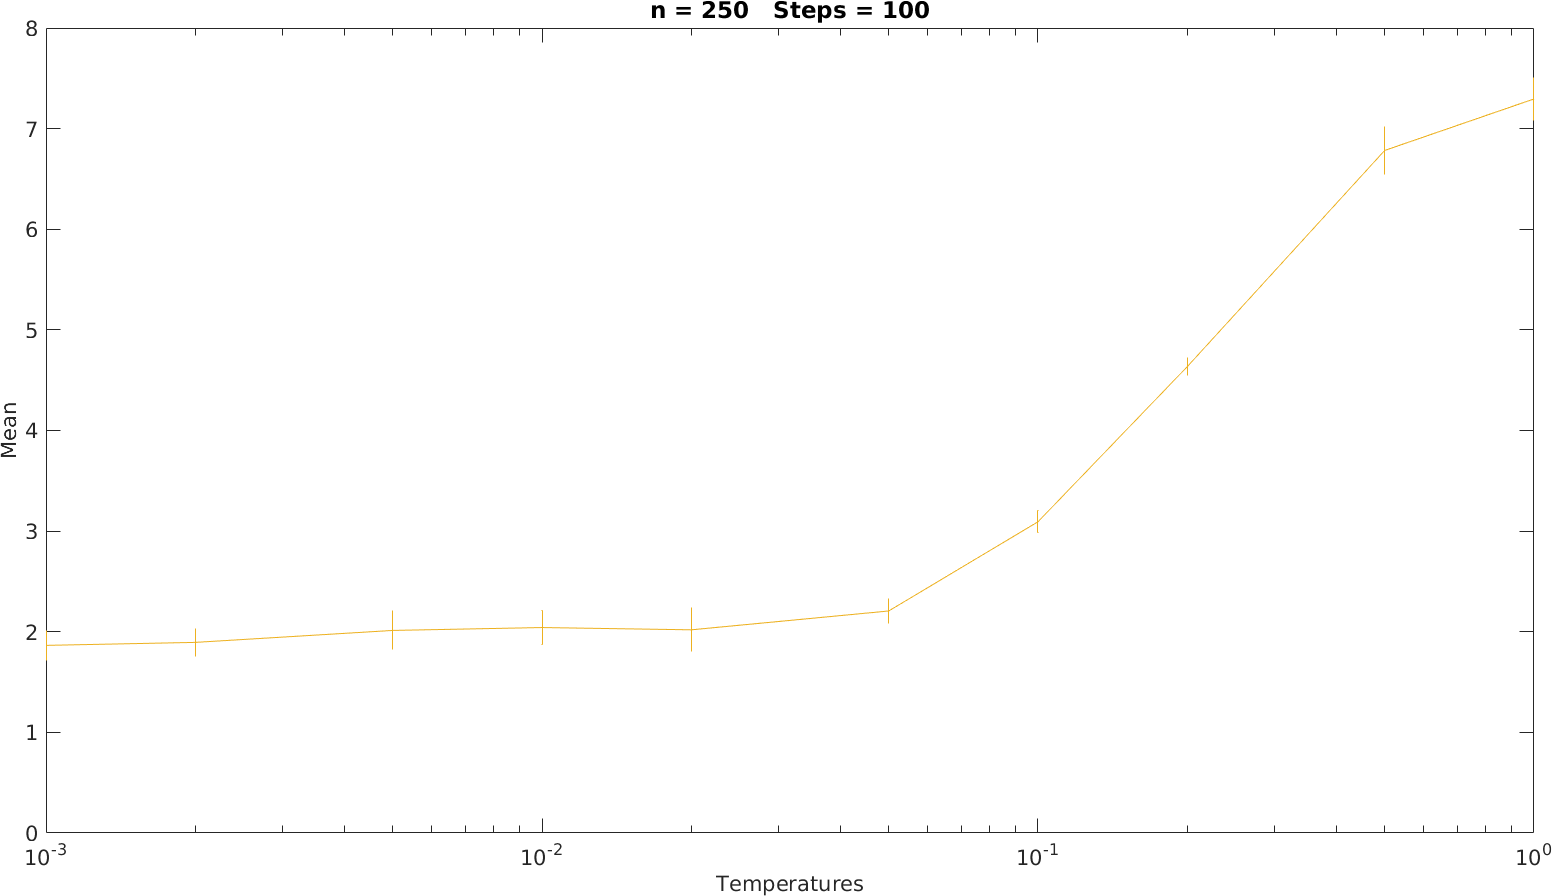
\includegraphics[width=\textwidth]{./Salesman/n250s100}} \\
Increasing the amount of cities from 50 to 250 also shows an increase of the mean (the y-axis has increased to 8 from 4 to accomodate for the mean) and the standard deviation. It also shows something odd with the standard deviation. At the higher temperatures, it seems to be quite small compared to the standard deviation at lower temperatures. It is possible that the cause for this is the high degree of random route-changes. The high temperature results is a less greedy algorithm, and thus the distance needs to decrease less. However, this is true for the other plots as well, as shown with the large means at high temperatures. But here, because the number of steps are not nearly enough for 500 cities, very little progress is made. That combined with the lack of direction (i.e., high temperature), results in a somewhat constant distance, which then leads to a small standard deviation.\\

\makebox[\textwidth]{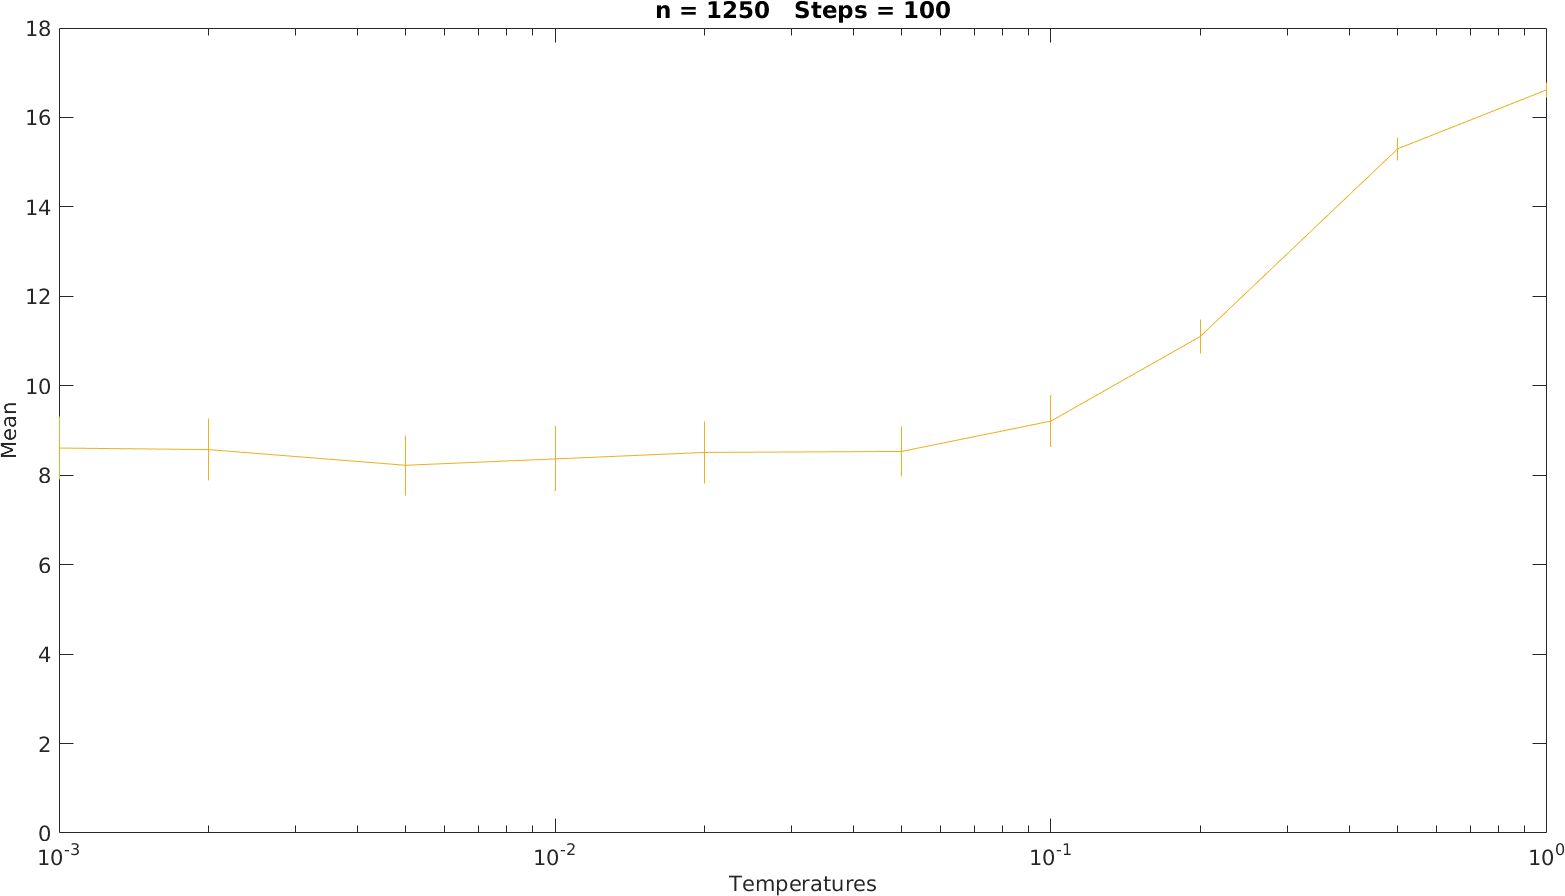
\includegraphics[width=\textwidth]{./Salesman/n1250s100}} \\

\makebox[\textwidth]{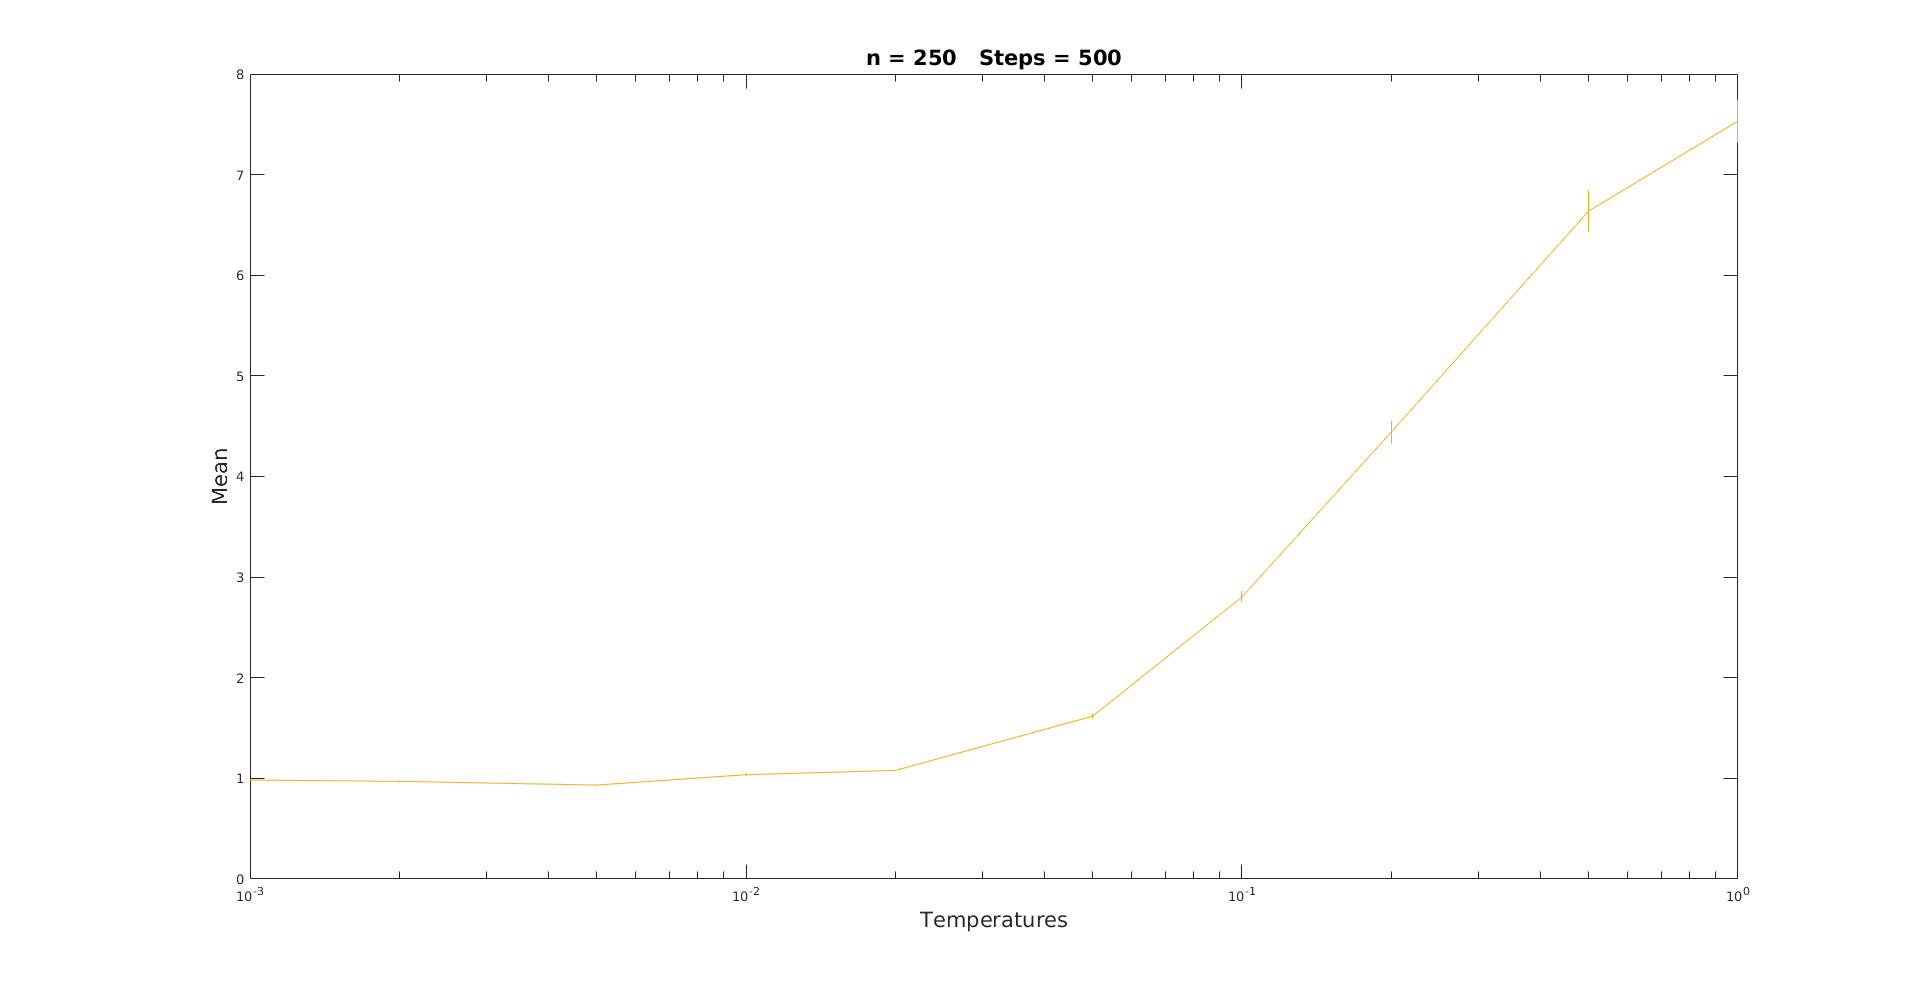
\includegraphics[width=\textwidth]{./Salesman/n250s500}} \\

\makebox[\textwidth]{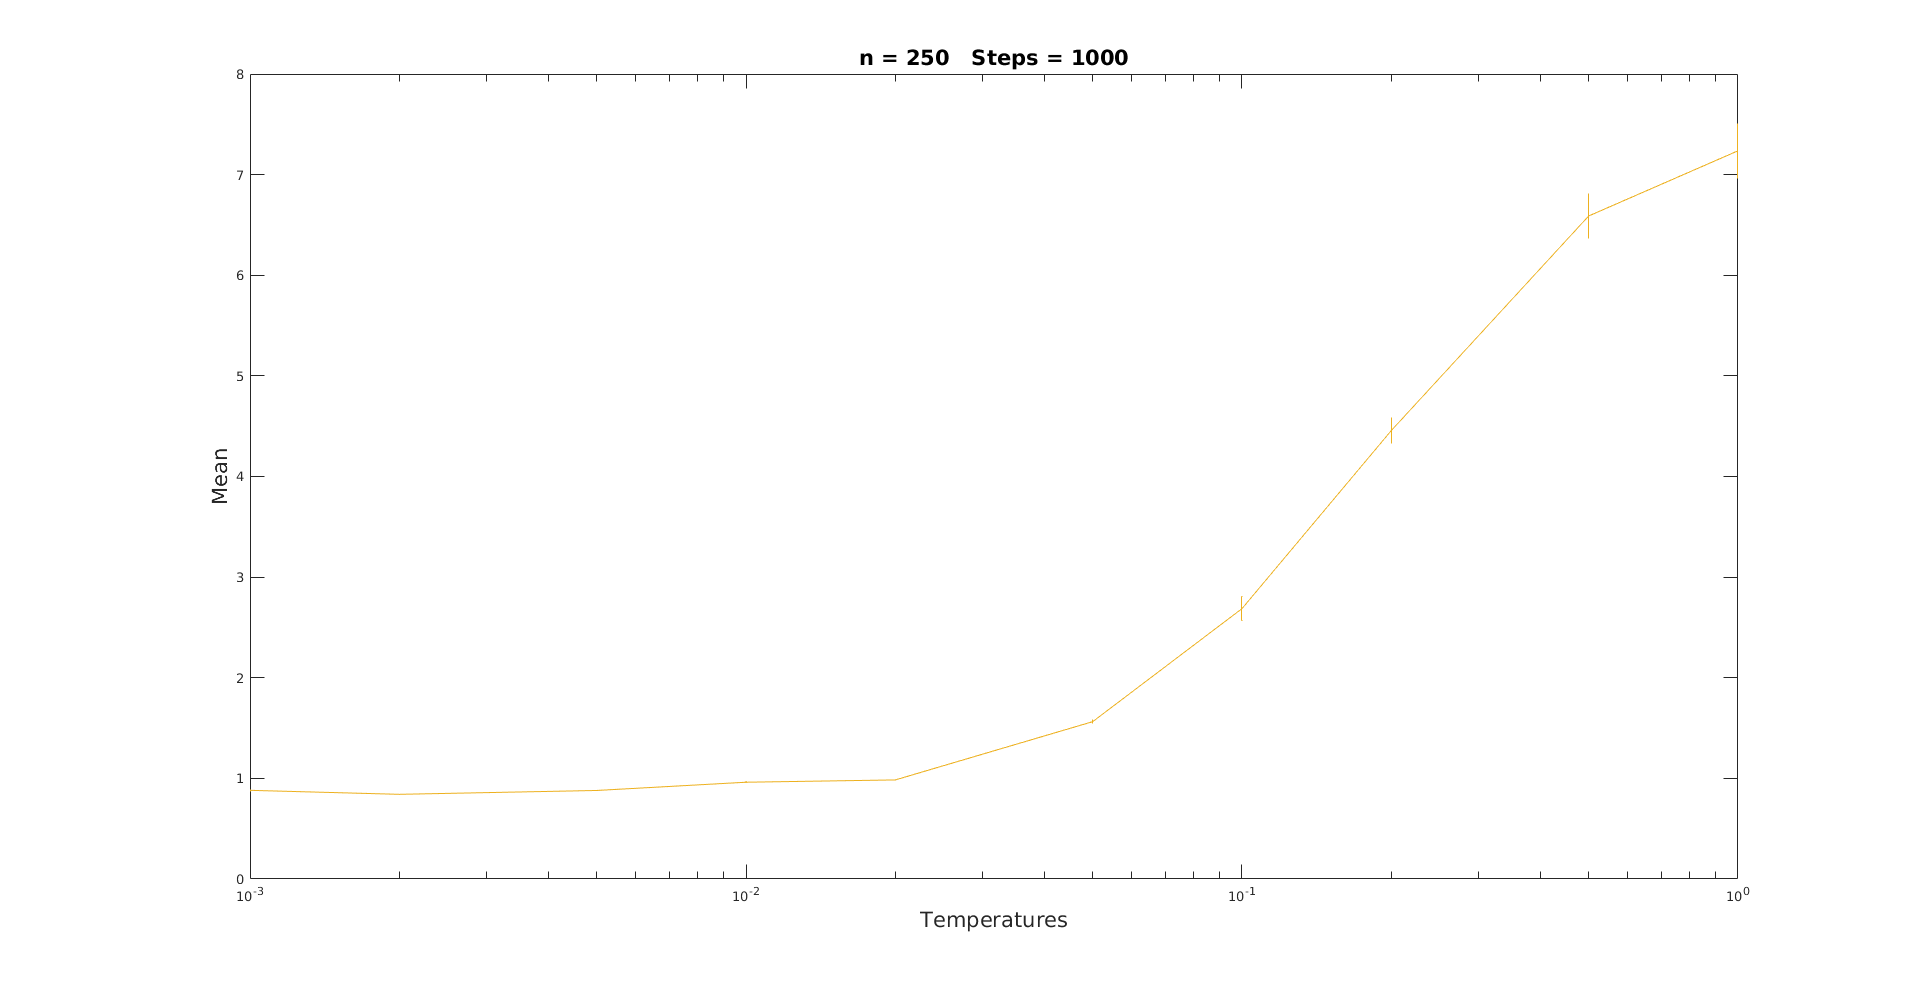
\includegraphics[width=\textwidth]{./Salesman/n250s1000}} \\

\section{T-Dependance}
In every plot seen, a lower temperature resulted in a shorter distance. Running the algorithm with a lower temperature makes it more greedy. In a sense, it encourages the algorithm to go for the shorter distances. When the temperature is higher, this push for a short distance is made a lot less, thus resulting in a longer distance. Apparently, local minima do not seem to be an issue even with very small values for the temperature.

\section{Work done}
The MatLab code was written by Sander and refactored by Wessel. 
This code was then used to generate several plots, as done by Wessel. Sander wrote the text for the document, with verbal input and suggestions from Wessel.
\end{document}